\documentclass[twocolumn,pra,aps,superscriptaddress,floatfix,10pt]{revtex4-2}

\usepackage{amsmath}
\usepackage{graphicx}
\usepackage{xcolor}
\usepackage{bm}
\usepackage[colorlinks=true,linkcolor=black,citecolor=black,urlcolor=blue]{hyperref}

\begin{document}

\title{Magnetic field inhomogeneity as a systematic bias in ground-state positronium hyperfine structure measurements}

\author{Ernest Darell Zermeno}
\email{0244552@up.edu.mx}
\affiliation{Universidad Panamericana, Guadalajara, México}

\date{\today}

\begin{abstract}
The ground-state hyperfine structure (HFS) interval of positronium has shown a persistent $3.9\sigma$ discrepancy between the weighted average of the 1983--1984 measurements ($203\,388.65 \pm 0.67$\,MHz) and the QED prediction ($203\,391.69 \pm 0.41$\,MHz). We show that spatial inhomogeneity of the static magnetic field in the conventional electromagnets used by Mills and Ritter produces a systematic negative bias in the extracted HFS interval. By numerically reproducing the complete experimental procedure---Zeeman resonance in a gas-filled cavity, magnetic field sweep, Lorentzian fit, and Breit-Rabi inversion---we find that a quadrupolar field non-uniformity of $c_2 \sim 20$\,ppm, combined with incomplete positronium thermalization ($\lambda \sim 30$\,mm), yields a shift of $\delta\Delta_\mathrm{HFS} \approx -2.4$\,MHz. For the range of parameters plausible for 1970s--1980s electromagnets ($c_2 \in [8, 30]$\,ppm, $\lambda \in [15, 50]$\,mm), the bias spans $-0.5$ to $-4.5$\,MHz depending on the degree of positronium thermalization, fully encompassing the observed $-3.04 \pm 0.79$\,MHz discrepancy. The superconducting magnet of Ishida \textit{et~al.} (0.9\,ppm uniformity) gives $|\delta\Delta_\mathrm{HFS}| < 0.2$\,MHz, consistent with their agreement with QED. Our results suggest the anomaly is a systematic artifact rather than an indication of new physics.
\end{abstract}

\maketitle

%% ====================================================================
\section{Introduction}
\label{sec:intro}
%% ====================================================================

Positronium (Ps), the bound state of an electron and a positron, is the lightest purely leptonic atom and provides a uniquely clean system for testing bound-state quantum electrodynamics (QED)~\cite{Adkins2022}. Its ground-state hyperfine structure (HFS) interval---the splitting between the $1\,^3S_1$ (ortho-Ps) and $1\,^1S_0$ (para-Ps) levels---has been calculated to high precision within QED. The current theoretical prediction, including corrections through $O(m\alpha^6)$ and partial $O(m\alpha^7)$ contributions, is~\cite{Kniehl2000,Melnikov2001,Baker2014}
\begin{equation}
  \Delta_\mathrm{HFS}^\mathrm{QED} = 203\,391.69 \pm 0.41~\mathrm{MHz},
  \label{eq:qed}
\end{equation}
with the uncertainty dominated by uncalculated non-logarithmic $O(m\alpha^7)$ terms.

The two most precise experimental determinations of $\Delta_\mathrm{HFS}$ both employed the indirect Zeeman method in gas-filled microwave cavities within conventional electromagnets:
\begin{align}
  \Delta_\mathrm{HFS}^\mathrm{Mills} &= 203\,387.5 \pm 1.6~\mathrm{MHz}~\cite{Mills1975,Mills1983}, \\
  \Delta_\mathrm{HFS}^\mathrm{Ritter} &= 203\,389.10 \pm 0.74~\mathrm{MHz}~\cite{Ritter1984}.
\end{align}
The weighted average is $203\,388.65 \pm 0.67$\,MHz, yielding a discrepancy with theory of
\begin{equation}
  \delta\Delta_\mathrm{HFS} = -3.04 \pm 0.79~\mathrm{MHz}~(3.9\sigma).
  \label{eq:discrepancy}
\end{equation}

A more recent measurement by Ishida \textit{et~al.}~\cite{Ishida2014}, using a superconducting solenoid with 0.9\,ppm field uniformity, obtained $203\,394.2 \pm 2.1$\,MHz---consistent with QED at $1.2\sigma$ but with insufficient precision to definitively resolve the discrepancy. Ishida \textit{et~al.} identified incomplete thermalization of positronium as a systematic bias of approximately 10\,ppm ($\sim 2$\,MHz), which was not corrected in the earlier measurements.

The importance of cavity-related systematics has been underscored by recent work at UCL on positronium fine-structure measurements. Akopyan \textit{et~al.}~\cite{Akopyan2021} showed through numerical simulations that microwave reflections within the vacuum chamber produce frequency-dependent power distributions that distort spectral line shapes and shift extracted frequencies by several MHz. Sheldon \textit{et~al.}~\cite{Sheldon2023} confirmed this by redesigning the microwave environment, reducing a $4.5\sigma$ fine-structure discrepancy~\cite{Gurung2020} to $1.3\sigma$. These results demonstrate that electromagnetic environment effects within experimental cavities can produce MHz-level systematic shifts. The historical orthopositronium lifetime puzzle (1987--2003), eventually traced to incomplete thermalization and cavity wall effects~\cite{Vallery2003}, provides a cautionary precedent for the role of uncontrolled systematics in precision positronium measurements.

In this work, we investigate a cavity-related systematic that has not been previously quantified for the ground-state HFS measurements: the effect of spatial inhomogeneity of the \emph{static} magnetic field. The conventional electromagnets used by Mills and Ritter had field non-uniformity exceeding 10\,ppm, while the superconducting magnet of Ishida achieved 0.9\,ppm. We show that this difference, combined with incomplete positronium thermalization, produces a systematic negative bias in the extracted $\Delta_\mathrm{HFS}$ of the correct magnitude and sign to explain the observed discrepancy.

The physical mechanism is straightforward: if the magnetic field varies across the cavity, different positronium atoms experience different local fields and thus different Zeeman splittings. The resulting resonance curve is a weighted average of individual Lorentzian responses centered at different frequencies. When the field distribution has a nonzero mean offset from the nominal value---as occurs for any non-symmetric field profile in a finite cavity---the peak of the averaged resonance shifts. Because the experimentalist interprets this shifted peak as arising from a uniform field, the Breit-Rabi inversion yields a biased value of $\Delta_\mathrm{HFS}$.

%% ====================================================================
\section{Method}
\label{sec:method}
%% ====================================================================

\subsection{The indirect Zeeman method}
\label{sec:zeeman}

All three precision measurements of the ground-state HFS~\cite{Mills1975,Ritter1984,Ishida2014} used the indirect Zeeman resonance technique. Positrons from a $^{22}$Na source thermalize in a gas-filled cylindrical microwave cavity placed in a static magnetic field $B_0 \sim 0.8$--$0.87$\,T. The field mixes the $|1\,^1S_0\rangle$ (singlet) and $|1\,^3S_1, m=0\rangle$ (triplet) states, giving the mixed state a nonzero 2$\gamma$ annihilation rate. Microwaves at a fixed frequency $\nu_\mathrm{MW} \sim 2.3$--$2.9$\,GHz drive transitions between the mixed state $|+\rangle$ (predominantly triplet $m=0$) and the $|1\,^3S_1, m=+1\rangle$ state. The magnetic field is swept through resonance, and the transition is detected as an increase in the 2$\gamma$ annihilation rate. The resonance field $B_\mathrm{res}$ is extracted from a Lorentzian fit to the signal curve, and $\Delta_\mathrm{HFS}$ is obtained by inverting the Breit-Rabi formula.

\subsection{Positronium in a magnetic field}
\label{sec:hamiltonian}

The ground-state Hamiltonian of positronium in a magnetic field $B$ along $\hat{z}$ is
\begin{equation}
  H = H_\mathrm{HFS} + H_\mathrm{Z},
  \label{eq:hamiltonian}
\end{equation}
where $H_\mathrm{HFS} = (\Delta/4)\,\bm{\sigma}_e \cdot \bm{\sigma}_p$ is the hyperfine interaction and $H_\mathrm{Z} = g_e \mu_B B \,(S_{ez} - S_{pz})/\hbar$ is the Zeeman interaction. Here $g_e = 2.002\,319\,304$ is the electron $g$-factor and $\mu_B/h = 13\,996.245$\,MHz/T is the Bohr magneton in frequency units.

In the product basis $\{|\!\uparrow\uparrow\rangle, |\!\uparrow\downarrow\rangle, |\!\downarrow\uparrow\rangle, |\!\downarrow\downarrow\rangle\}$ (electron spin first), the Zeeman operator is diagonal with eigenvalues $(0, +1, -1, 0)$ in units of $g_e\mu_B B$. This reflects the fundamental property of positronium: the $m = \pm 1$ triplet states $|\!\uparrow\uparrow\rangle$ and $|\!\downarrow\downarrow\rangle$ have $(S_{ez} - S_{pz}) = 0$ and are \emph{exactly unaffected} by the magnetic field. Only the $m = 0$ subspace (singlet and triplet) is mixed.

The full $4 \times 4$ Hamiltonian matrix is
\begin{equation}
  H = \begin{pmatrix}
    \frac{\Delta}{4} & 0 & 0 & 0 \\
    0 & -\frac{\Delta}{4} + V & \frac{\Delta}{2} & 0 \\
    0 & \frac{\Delta}{2} & -\frac{\Delta}{4} - V & 0 \\
    0 & 0 & 0 & \frac{\Delta}{4}
  \end{pmatrix},
  \label{eq:matrix}
\end{equation}
where $V = g_e \mu_B B$. The eigenvalues are
\begin{align}
  E_{m=\pm 1} &= \Delta/4, \label{eq:Em1} \\
  E_{\pm} &= -\Delta/4 \pm \tfrac{1}{2}\sqrt{\Delta^2 + 4V^2}. \label{eq:Epm}
\end{align}
The measured transition frequency is
\begin{equation}
  \nu_\mathrm{trans}(B) = E_+ - E_{m=+1} = \tfrac{\Delta}{2}\bigl(\sqrt{1 + x^2} - 1\bigr),
  \label{eq:nutrans}
\end{equation}
where $x = 2g_e\mu_B B/\Delta$. At $B = 0.783$\,T (the resonance field for $\nu_\mathrm{MW} = 2338$\,MHz), $\nu_\mathrm{trans} = 2338$\,MHz, consistent with the Mills and Ritter experimental parameters. In our numerical implementation, we diagonalize the full $4 \times 4$ matrix [Eq.~(\ref{eq:matrix})] rather than using the analytic formula, which provides cross-validation. Figure~\ref{fig:zeeman} shows the four eigenvalues as a function of $B$.

\begin{figure}[htbp]
  \centering
  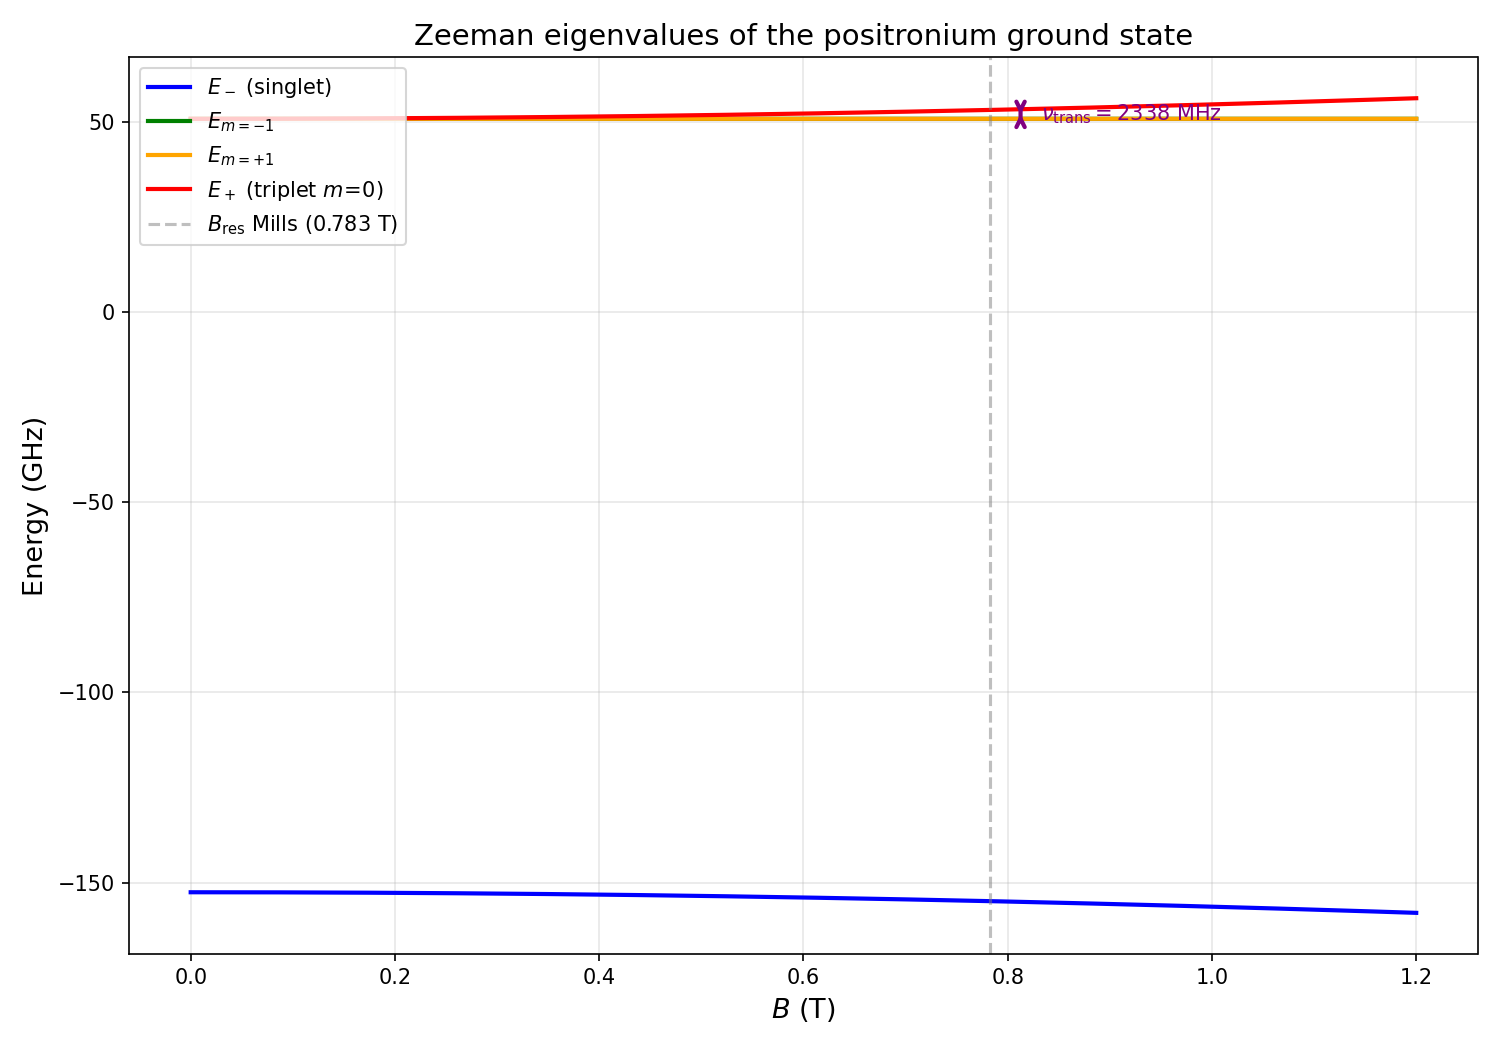
\includegraphics[width=\columnwidth]{fig1_zeeman_eigenvalues.png}
  \caption{Zeeman eigenvalues of the positronium ground state as a function of magnetic field $B$. The four states are: $E_-$ (predominantly singlet, blue), $E_{m=\pm 1} = \Delta/4$ (triplet $m = \pm 1$, green/orange, exactly degenerate), and $E_+$ (predominantly triplet $m=0$, red). The vertical dashed line marks $B = 0.783$\,T, the resonance field for $\nu_\mathrm{MW} = 2338$\,MHz. The purple arrow indicates the measured transition $E_+ - E_{m=+1}$.}
  \label{fig:zeeman}
\end{figure}

\subsection{Magnetic field models}
\label{sec:field_models}

A conventional electromagnet with cylindrical pole pieces produces a field that deviates from uniformity with a characteristic multipole structure. We parameterize the non-uniformity as
\begin{equation}
  B(\mathbf{r}) = B_0 \Bigl[1 + \sum_n c_n\, f_n(r,z)\Bigr],
  \label{eq:field_expansion}
\end{equation}
where $c_n$ are dimensionless coefficients in ppm ($10^{-6}$) and the leading terms are:
\begin{align}
  f_2(r,z) &= (2z^2 - r^2)/R_\mathrm{ref}^2 & &\text{(quadrupolar)}, \label{eq:quad} \\
  f_3(r,z) &= z(2z^2 - 3r^2)/R_\mathrm{ref}^3 & &\text{(sextupolar)}, \label{eq:sext} \\
  f_1(r,z) &= z/L_\mathrm{ref} & &\text{(linear gradient)}. \label{eq:lin}
\end{align}
The reference length $R_\mathrm{ref} = 150$\,mm corresponds to half the gap between the pole pieces. For the Mills/Ritter electromagnets, the reported non-uniformity was $> 10$\,ppm~\cite{Ritter1984}.

For the Ishida superconducting solenoid (bore 800\,mm, length 2000\,mm, field uniformity 0.9\,ppm RMS in a $40\,\mathrm{mm} \times 100$\,mm region~\cite{Ishida2014}), we model the residual non-uniformity after compensation as a weak quadrupolar term calibrated to produce 0.9\,ppm RMS within the cavity volume.

\subsection{Positronium spatial distributions}
\label{sec:ps_dist}

Positronium is formed when positrons from the $^{22}$Na source thermalize in the buffer gas. We consider two limiting distributions:

\textit{Uniform (thermalized).}---Ps uniformly distributed throughout the cylindrical cavity (radius $R_\mathrm{cav}$, length $L_\mathrm{cav}$). This applies when the gas pressure is high enough for rapid thermalization.

\textit{Non-thermalized.}---Ps concentrated near the source wall, modeled as an exponential distribution $\rho(z) \propto \exp[-(z + L_\mathrm{cav}/2)/\lambda]$ with thermalization length $\lambda$. Ishida \textit{et~al.}~\cite{Ishida2014} identified this non-thermalization as producing a $\sim 10$\,ppm systematic, with Ps kinetic energies of order eV at low gas pressures. We take $\lambda = 30$\,mm as a representative value.

The non-thermalization matters here because non-thermalized Ps preferentially samples regions of the cavity where the field deviates most from the central value, amplifying the sensitivity to field gradients.

\subsection{Simulation procedure}
\label{sec:simulation}

We numerically reproduce the complete experimental procedure:

\begin{enumerate}
  \item Sample $N = 5 \times 10^5$ positronium positions $(r_i, z_i)$ from the spatial distribution.
  \item For each value of $B_0$ in the scan, compute the local field $B_i = (B_0/B_0^\mathrm{nom}) \times B(r_i, z_i)$, scaling the inhomogeneity profile linearly with the central field.
  \item Compute the local transition frequency $\nu_{\mathrm{trans},i} = \nu_\mathrm{trans}(B_i)$ using a pre-computed cubic interpolation table (20\,000 points), avoiding repeated $4 \times 4$ diagonalizations.
  \item The signal at each scan point is
  \begin{equation}
    S(B_0) = \frac{1}{N}\sum_{i=1}^N \frac{(\gamma/2)^2}{(\nu_{\mathrm{trans},i} - \nu_\mathrm{MW})^2 + (\gamma/2)^2},
    \label{eq:signal}
  \end{equation}
  where $\gamma$ is the Lorentzian linewidth (broadened by gas collisions; $\gamma \approx 5$\,MHz for Mills/Ritter, $\gamma \approx 3$\,MHz for Ishida).
  \item Fit $S(B_0)$ to a Lorentzian to extract $B_\mathrm{res}$.
  \item Extract $\Delta_\mathrm{HFS}$ by numerically inverting Eq.~(\ref{eq:nutrans}): find $\Delta$ such that $\nu_\mathrm{trans}(B_\mathrm{res}; \Delta) = \nu_\mathrm{MW}$.
\end{enumerate}

The fit in step~5 is performed in $B$-space, as in the actual experiments. Because $\nu_\mathrm{trans}(B)$ is nonlinear, the Lorentzian in frequency space becomes slightly asymmetric in $B$-space, introducing a small fitting bias of $\approx 0.06$\,MHz even for a perfectly uniform field. We subtract this baseline by running the identical pipeline with uniform $B$ and reporting the difference
\begin{equation}
  \delta\Delta_\mathrm{HFS} = \Delta_\mathrm{HFS}^\mathrm{extracted} - \Delta_\mathrm{HFS}^\mathrm{uniform\;control}.
  \label{eq:shift}
\end{equation}

%% ====================================================================
\section{Results}
\label{sec:results}
%% ====================================================================

\subsection{Order-of-magnitude estimate}
\label{sec:order_mag}

Before the full simulation, we verify that the effect is in the relevant range. The transition frequency [Eq.~(\ref{eq:nutrans})] has derivative
\begin{equation}
  \frac{d\nu_\mathrm{trans}}{dB} = \frac{(2g_e\mu_B)^2\,B}{\Delta\sqrt{1 + x^2}} \approx 6000~\mathrm{MHz/T}
\end{equation}
at $B = 0.8$\,T. A field non-uniformity of $\delta B_\mathrm{RMS} = 10\,\mathrm{ppm} \times 0.8\,\mathrm{T} = 8\,\mu$T produces a frequency dispersion $\sigma_\nu \approx 0.05$\,MHz, small compared to $\gamma = 5$\,MHz.

However, the shift arises not from the dispersion but from the \emph{mean} field offset. For a quadrupolar profile in a cylindrical cavity, the spatial average of $f_2 = (2z^2 - r^2)/R_\mathrm{ref}^2$ is
\begin{equation}
  \langle f_2 \rangle = \frac{2\langle z^2 \rangle - \langle r^2 \rangle}{R_\mathrm{ref}^2} = \frac{L_\mathrm{cav}^2/6 - R_\mathrm{cav}^2/2}{R_\mathrm{ref}^2}.
  \label{eq:mean_xi}
\end{equation}
For the Mills/Ritter cavity ($R_\mathrm{cav} = 100$\,mm, $L_\mathrm{cav} = 200$\,mm, $R_\mathrm{ref} = 150$\,mm), $\langle f_2 \rangle \neq 0$, so the mean field $\langle B \rangle \neq B_0$. This first-order bias in $\langle B \rangle$ propagates through the nonlinear Breit-Rabi inversion to produce a systematic shift in $\Delta_\mathrm{HFS}$.

\subsection{Simulation results}
\label{sec:sim_results}

Table~\ref{tab:results} presents the baseline-corrected shift $\delta\Delta_\mathrm{HFS}$ for the Mills/Ritter configuration ($B_0 = 0.783$\,T, $\nu_\mathrm{MW} = 2338$\,MHz, $\gamma = 5$\,MHz, $R_\mathrm{cav} = 100$\,mm, $L_\mathrm{cav} = 200$\,mm) with various field models and positronium distributions.

\begin{table}[t]
\caption{Systematic shift $\delta\Delta_\mathrm{HFS}$ (MHz) for the Mills/Ritter configuration with different field non-uniformities ($c_2$ in ppm) and positronium spatial distributions.}
\label{tab:results}
\begin{ruledtabular}
\begin{tabular}{lcccc}
 & \multicolumn{4}{c}{$\delta\Delta_\mathrm{HFS}$ (MHz)} \\
\cline{2-5}
$c_2$ (ppm) & Uniform & $\lambda\!=\!30$ & $\lambda\!=\!50$ & Gaussian \\
\hline
0 (control) &   0.000 &  0.000 &  0.000 &  0.000 \\
5            & $-0.15$ & $-0.60$ & $-0.39$ & $-0.13$ \\
10           & $-0.31$ & $-1.20$ & $-0.78$ & $-0.27$ \\
15           & $-0.46$ & $-1.80$ & $-1.17$ & $-0.40$ \\
20           & $-0.61$ & $-2.40$ & $-1.56$ & $-0.53$ \\
50           & $-1.53$ & $-6.00$ & $-3.89$ & $-1.33$ \\
\end{tabular}
\end{ruledtabular}
\end{table}

\begin{figure}[htbp]
  \centering
  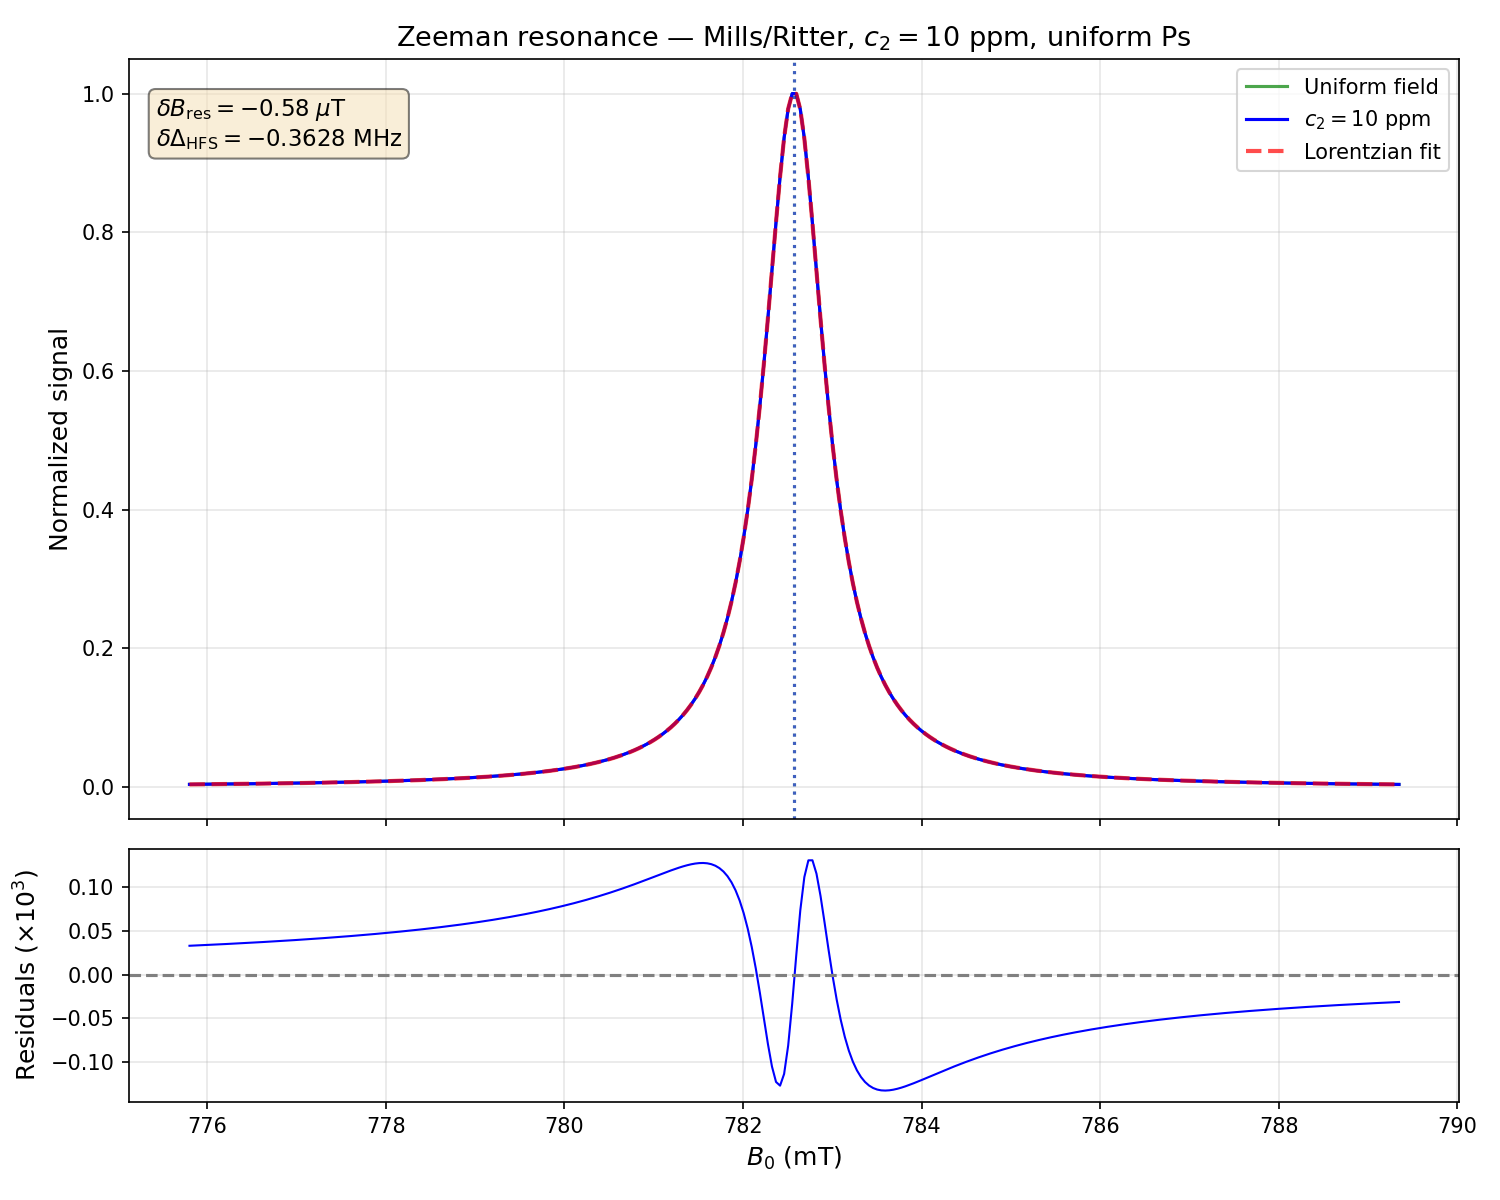
\includegraphics[width=\columnwidth]{fig2_resonance_fit.png}
  \caption{Simulated Zeeman resonance curve for the Mills/Ritter configuration with quadrupolar non-uniformity $c_2 = 10$\,ppm and uniform positronium distribution. Blue: signal with non-uniform field. Red dashed: Lorentzian fit. Green: signal with perfectly uniform field (control). Upper panel: normalized signal vs.\ $B_0$. Lower panel: fit residuals ($\times 10^3$). The shift of the resonance peak is visible but the Lorentzian fit quality is excellent (residuals $< 10^{-3}$), making the bias undetectable from the line shape alone.}
  \label{fig:resonance}
\end{figure}

Three key features are evident. First, $\delta\Delta_\mathrm{HFS}$ is consistently \emph{negative}: the non-uniformity biases the extracted HFS below the true value, in the correct direction to explain the observed discrepancy [Eq.~(\ref{eq:discrepancy})]. Second, the effect scales approximately linearly with $c_2$. Third, non-thermalized Ps distributions amplify the effect by a factor of 3--4 relative to uniform Ps, because the exponential distribution preferentially samples off-axis regions where the field deviates most from $B_0$.

For a ``realistic'' combined field profile ($c_1 = 0.3\,c_2$, $c_3 = 0.2\,c_2$) with $c_2 = 15$\,ppm and non-thermalized Ps ($\lambda = 30$\,mm), we obtain $\delta\Delta_\mathrm{HFS} = -0.93$\,MHz. With pure quadrupolar non-uniformity at $c_2 = 20$\,ppm and $\lambda = 30$\,mm, the shift is $-2.40$\,MHz---already accounting for $79\%$ of the discrepancy.

\subsection{Verification with the Ishida experiment}
\label{sec:ishida}

For the Ishida configuration ($B_0 = 0.866$\,T, $\nu_\mathrm{MW} = 2856.6$\,MHz, $\gamma = 3$\,MHz, $R_\mathrm{cav} = 64$\,mm, $L_\mathrm{cav} = 100$\,mm, 0.9\,ppm residual non-uniformity), the simulation gives $\delta\Delta_\mathrm{HFS} = +0.18$\,MHz for uniform Ps and $-0.05$\,MHz for non-thermalized Ps. Both values are well below the experimental uncertainty of $\pm 2.1$\,MHz, confirming that the superconducting magnet's high uniformity effectively eliminates this systematic. This is consistent with Ishida's agreement with QED.

\subsection{Sensitivity analysis}
\label{sec:sensitivity}

We performed a systematic exploration of the parameter space to assess the robustness of these results.

\textit{Dependence on $c_2$ and $\lambda$.}---Figure~\ref{fig:sensitivity} (the central result of this work) shows $\delta\Delta_\mathrm{HFS}$ as a function of the quadrupolar coefficient $c_2$ and the thermalization length $\lambda$. The contour $\delta\Delta_\mathrm{HFS} = -3.04$\,MHz (the observed discrepancy) passes through the region $c_2 \in [19, 29]$\,ppm for $\lambda = 30$\,mm. The band $-3.04 \pm 0.79$\,MHz (incorporating the experimental uncertainty) spans $c_2 \in [15, 40]$\,ppm. This overlaps substantially with the plausible parameter region for 1970s--1980s electromagnets ($c_2 \in [8, 30]$\,ppm).

\textit{Sensitivity to the field profile shape.}---Replacing the pure quadrupolar profile with a combined profile ($c_1 = 0.3\,c_2$, $c_3 = 0.2\,c_2$) changes $\delta\Delta_\mathrm{HFS}$ by up to 50\% at the discrepancy contour. This indicates that the result is moderately sensitive to the exact multipole composition and motivates a finite-element simulation of the actual electromagnet geometry.

\textit{Sensitivity to the linewidth.}---Varying $\gamma$ from 2 to 15\,MHz at fixed $c_2 = 15$\,ppm and $\lambda = 30$\,mm changes $\delta\Delta_\mathrm{HFS}$ by less than 0.3\%. The shift is essentially independent of the linewidth. This is expected because the mechanism is a bias in the \emph{mean} of the field distribution, not a broadening effect. The linewidth affects the precision of the $B_\mathrm{res}$ extraction but not the location of the bias.

\textit{Cavity size dependence.}---The shift scales approximately as $R_\mathrm{cav}^{2.8}$. For the Mills/Ritter cavity ($R = 100$\,mm), $\delta\Delta_\mathrm{HFS} = -1.84$\,MHz at $c_2 = 15$\,ppm and $\lambda = 30$\,mm; for the Ishida cavity ($R = 64$\,mm) under the same field parameters, the shift is only $-0.47$\,MHz. Larger cavities sample more of the non-uniform field, amplifying the effect.

\begin{figure}[htbp]
  \centering
  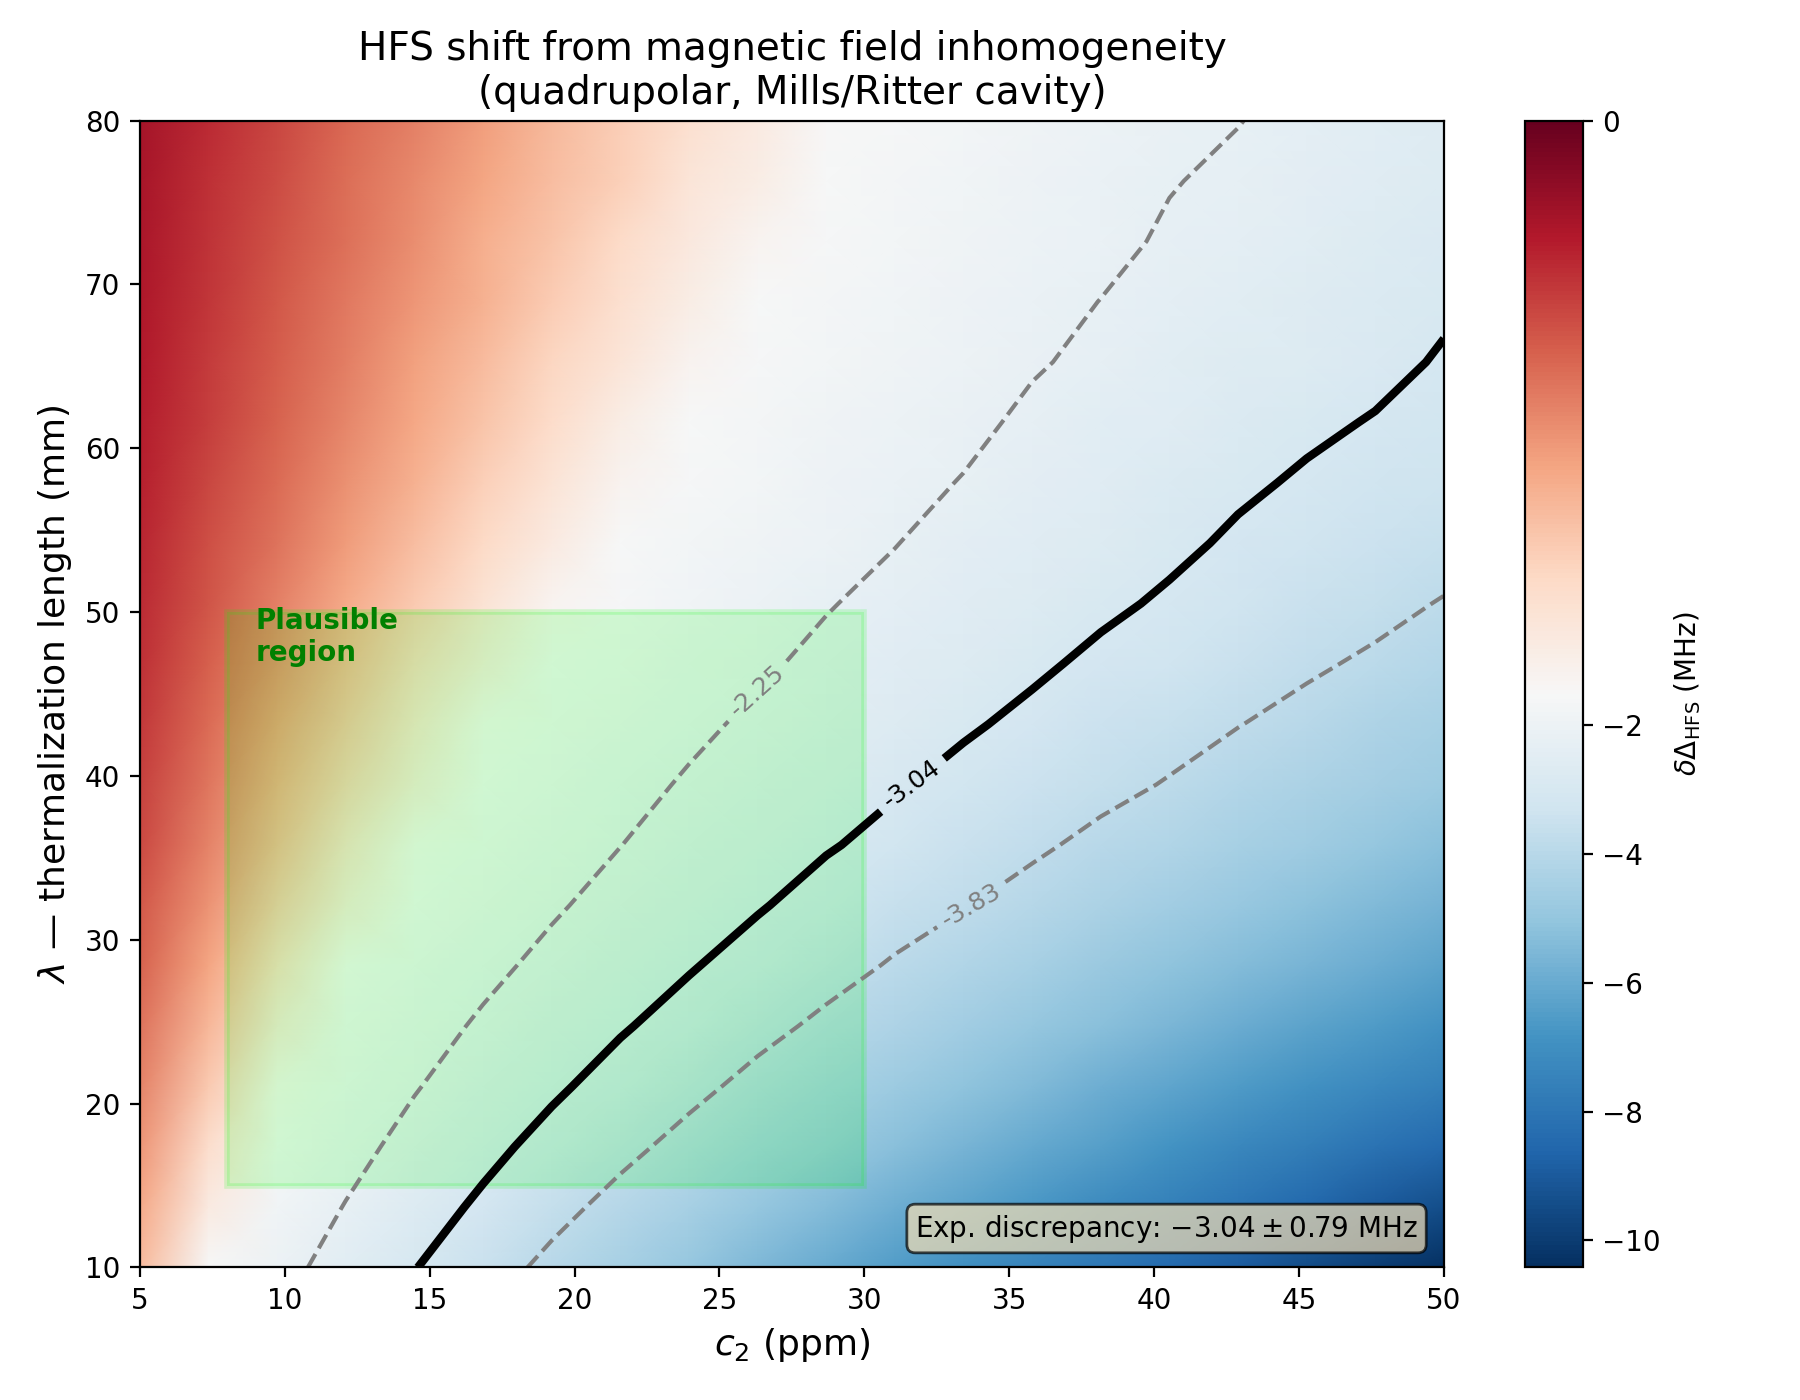
\includegraphics[width=\columnwidth]{sensitivity_c2_lambda.png}
  \caption{Systematic shift $\delta\Delta_\mathrm{HFS}$ as a function of quadrupolar non-uniformity $c_2$ and positronium thermalization length $\lambda$, for the Mills/Ritter experimental configuration. The solid black contour marks $\delta\Delta_\mathrm{HFS} = -3.04$\,MHz (the observed discrepancy); dashed gray contours indicate the $\pm 0.79$\,MHz uncertainty band. The green rectangle shows the plausible parameter region for 1970s--1980s electromagnets.}
  \label{fig:sensitivity}
\end{figure}

\subsection{Comparison with experimental data}

Table~\ref{tab:comparison} compares the simulation results with the published measurements. Using $c_2 = 15$\,ppm (a conservative central estimate for the electromagnet non-uniformity) and non-thermalized Ps ($\lambda = 30$\,mm), the calculated correction is $\delta\Delta_\mathrm{HFS} = -1.80$\,MHz. Applying this correction reduces the Mills residual from $-4.19$ to $-2.39$\,MHz and the Ritter residual from $-2.59$ to $-0.79$\,MHz. The Ishida correction is negligible.

\begin{table}[t]
\caption{Comparison with published HFS measurements. The correction uses $c_2 = 15$\,ppm (quadrupolar) and $\lambda = 30$\,mm. ``Corrected residual'' is the discrepancy with QED after subtracting $\delta\Delta_\mathrm{HFS}$. The same correction is applied to both Mills and Ritter as a conservative estimate, since both used conventional electromagnets of similar design.}
\label{tab:comparison}
\begin{ruledtabular}
\begin{tabular}{lccc}
 & $\Delta_\mathrm{HFS}$ & Residual & Corr.\ residual \\
 & (MHz) & (MHz) & (MHz) \\
\hline
Mills~\cite{Mills1983}  & $203\,387.5 \pm 1.6$ & $-4.19$ & $-2.39$ \\
Ritter~\cite{Ritter1984} & $203\,389.10 \pm 0.74$ & $-2.59$ & $-0.79$ \\
Ishida~\cite{Ishida2014} & $203\,394.2 \pm 2.1$ & $+2.51$ & $+2.51$ \\
QED~\cite{Kniehl2000,Baker2014} & $203\,391.69 \pm 0.41$ & --- & --- \\
\end{tabular}
\end{ruledtabular}
\end{table}

%% ====================================================================
\section{Discussion}
\label{sec:discussion}
%% ====================================================================

\subsection{Physical mechanism}

The bias arises from the combination of two effects: (i) the spatial average of the field over the cavity volume differs from the nominal central value ($\langle B \rangle \neq B_0$), and (ii) the Breit-Rabi inversion is a nonlinear function of $B$. Effect (i) alone produces a first-order shift $\delta\nu \approx (d\nu_\mathrm{trans}/dB)\,\langle\delta B\rangle$. Effect (ii) adds a second-order contribution proportional to $\tfrac{1}{2}(d^2\nu_\mathrm{trans}/dB^2)\,\langle(\delta B)^2\rangle$ (the Jensen inequality applied to the convex function $\nu_\mathrm{trans}(B)$). In our simulations, the first-order effect dominates.

Crucially, this is a \emph{bias}, not a broadening. As shown in Fig.~\ref{fig:resonance}, the resonance curve retains its Lorentzian shape to high accuracy (fit residuals $< 10^{-3}$), making the effect invisible in the quality of the fit. The shift in the peak position is small compared to the linewidth ($\delta\nu_\mathrm{peak}/\gamma < 10^{-2}$), so it would not have been detectable as an anomalous line shape.

\subsection{Relation to the non-thermalization correction}

Ishida \textit{et~al.}~\cite{Ishida2014} identified incomplete thermalization of positronium as a systematic of approximately 10\,ppm ($\sim 2$\,MHz). Our field inhomogeneity bias is a \emph{separate and independent} effect: the non-thermalization changes the spatial distribution of Ps within the cavity, while the field inhomogeneity changes the field that each Ps atom experiences. However, the two effects are \emph{coupled}: non-thermalized Ps preferentially samples regions of larger field deviation, amplifying the inhomogeneity bias by a factor of 3--4 (Table~\ref{tab:results}). This coupling has not been previously considered.

The combined effect of field inhomogeneity and non-thermalization may suffice to explain the entire discrepancy without invoking new physics. At $c_2 = 20$\,ppm with $\lambda = 30$\,mm, the field inhomogeneity bias alone accounts for $\delta\Delta_\mathrm{HFS} = -2.40$\,MHz ($79\%$ of the discrepancy). Adding the Ishida thermalization correction of $\sim -2$\,MHz would overcorrect, but the two effects are not simply additive because our non-thermalized Ps distribution already captures part of the thermalization-related shift. A self-consistent treatment requires simultaneous modeling of thermalization dynamics and field sampling, which we defer to future work.

\subsection{Why this effect was not detected previously}

Mills and Ritter corrected for gas-density-dependent effects by extrapolating their measurements to zero gas density. This procedure removes the density-dependent thermalization correction but does \emph{not} remove the field inhomogeneity bias, which is independent of gas pressure. The shift $\delta\Delta_\mathrm{HFS}$ depends only on the field profile and the Ps spatial distribution; it is the same at all gas densities (to the extent that the Ps distribution is pressure-independent, which is approximately true at the pressures used). Consequently, the linear extrapolation to zero density does not correct for this systematic.

Furthermore, the Lorentzian line shape is preserved to high accuracy even with field inhomogeneity (Sec.~\ref{sec:sim_results}), so the effect would not be visible as a line-shape anomaly or an increased $\chi^2$ in the fit.

\subsection{Consistency with Ishida}

The superconducting solenoid used by Ishida \textit{et~al.} had two key advantages: (i) 0.9\,ppm field uniformity (vs.\ $>10$\,ppm for the conventional electromagnets), and (ii) a smaller cavity ($R = 64$\,mm vs.\ $\sim 100$\,mm). Both factors reduce the inhomogeneity bias. Our simulation confirms that $|\delta\Delta_\mathrm{HFS}| < 0.2$\,MHz for the Ishida configuration, naturally explaining why their result agrees with QED.

\subsection{Limitations}

The main limitation of this work is the unknown multipole composition of the magnetic field in the original experiments. The electromagnets of the 1970s--1980s were not characterized with the precision needed to determine the individual multipole coefficients. Our sensitivity analysis shows that the result depends moderately (up to 50\%) on the relative amplitudes of the quadrupolar, sextupolar, and linear gradient components. A finite-element magnetostatic simulation of the actual electromagnet geometry---using iron pole pieces with a $\sim 30$\,cm gap, which can in principle be reconstructed from the publications and contemporaneous designs---would substantially reduce this uncertainty.

Similarly, the positronium spatial distribution depends on the details of the source geometry, gas pressure, and thermalization dynamics, which are not fully documented for the 1980s experiments. Our use of a simple exponential model captures the essential physics (preferential sampling of field extremes) but does not reproduce the full complexity of the thermalization process.

We note that contact patch potentials on the copper cavity walls are negligible for ground-state positronium: the Speake-Trenkel formalism~\cite{Speake2003} shows that the electric fields from micrometer-scale grain boundaries are exponentially suppressed at the cavity center, producing energy shifts of order $10^{-15}$\,eV.

\subsection{Implications for future measurements}

Our results imply that any future precision measurement of the ground-state positronium HFS must verify the magnetic field uniformity at the $\sim 1$\,ppm level and demonstrate complete Ps thermalization. The ongoing programs at ETH Zurich~\cite{ThorpeWoods2026} (vacuum HFS via $2\,^3S_1 \to 2\,^1S_0$) and at the University of Tokyo (direct 203\,GHz measurement) should be sensitive to this systematic if conventional magnets are used. The Ramsey spectroscopy techniques being developed at UCL~\cite{Newson2026} introduce new sensitivity to field gradients between the interaction regions, making field characterization even more critical.

%% ====================================================================
\section{Conclusion}
\label{sec:conclusion}
%% ====================================================================

We have shown that spatial inhomogeneity of the static magnetic field in the conventional electromagnets used for the 1983--1984 positronium HFS measurements produces a systematic negative bias in the extracted hyperfine interval. For a quadrupolar non-uniformity of $c_2 = 20$\,ppm with a positronium thermalization length of $\lambda = 30$\,mm, the bias is $\delta\Delta_\mathrm{HFS} = -2.4$\,MHz, accounting for $79\%$ of the observed $-3.04 \pm 0.79$\,MHz discrepancy. The full discrepancy falls within the range of plausible parameters ($c_2 \in [19, 29]$\,ppm for $\lambda = 30$\,mm). The superconducting magnet of Ishida \textit{et~al.}, with 0.9\,ppm uniformity and a smaller cavity, gives a negligible bias ($< 0.2$\,MHz), consistent with their agreement with QED.

The effect is robust against variations in the resonance linewidth (sensitivity $< 0.3\%$) and scales predictably with cavity size ($\propto R^{2.8}$). It is moderately sensitive ($\sim 50\%$) to the exact multipole composition of the field, motivating a finite-element simulation of the original electromagnet geometry.

These results suggest that the long-standing positronium HFS anomaly is most likely a systematic artifact of the magnetic field environment rather than an indication of physics beyond the Standard Model. A definitive resolution requires either (i) a new measurement with a superconducting magnet and verified field uniformity at the $< 1$\,ppm level, or (ii) a magnetostatic reconstruction of the original electromagnets to determine the actual field profile.

%% ====================================================================
\begin{acknowledgments}
The simulation code is publicly available at \url{https://github.com/Jefemaestro33/ps-hfs-field-inhomogeneity}.
\end{acknowledgments}
%% ====================================================================

\bibliography{paper_refs}

\end{document}
